\par\Needspace{12\baselineskip}
\section{Comparaisons renforcées du cycle Q2}
\label{supp:q2-comparisons}

\textbf{Statut et séparation des preuves.} Les comparaisons MAUDE 2023--2025, CMS nursing 2023--2025 et Part D 2023--2024 présentées ici proviennent de nouveaux ajustements Q2 sur des entrées vérifiées puis préparées à nouveau; ce ne sont ni des rejeux des métriques historiques ni une correction rétroactive de RC2.2. Les cohortes et périodes avaient déjà été consultées : tous les résultats restent exploratoires, sans nouvelle confirmation indépendante, nouvel intervalle de confiance, bootstrap ou test de significativité. Les définitions, dénominateurs, scores et audits historiques de S1--S11 restent conservés à part. Le protocole fixe les grilles et la sélection avant les scores de test; la complétion d'une grille ne rend pas son test indépendant\cite{hgbq2methods,hgbcode}.

Le protocole JSON exact est livré sous \src{data/q2/q2_scientific_protocol_20261003.json}. Les preuves compactes sont rangées sous \src{data/q2/} par basename : \src{q2_maude_validation_20261003.json}, \src{q2_maude_comparison_20261003.json}, \src{q2_cms_comparison_20261003.json}, \src{q2_partd_comparison_20261003.json}, \src{q2_external_reuse_20261003.json}, \src{q2_partd_prospective_20261003.json}, \src{q2_partd_prospective_publication_20261003.json} et \src{q2_cycle_status_20261003.json}. Le snapshot de lecture du code est sous \src{vendor/q2/healthgraphbench/} et \src{scripts/q2/}; il est rattaché au commit de provenance \src{6b4ae00ebc4b701d757260616ccb0df16f51467b}. Les runs consignent séparément les sources réellement consommées : validation MAUDE \src{abf13e3bbb279909c4633fd0dd7ed95231980129}, complétion MAUDE \src{ae648fed26bd87d0a731a0cb1fd8d0a4bee4c30a}, CMS \src{3e7d548800cbbfd317d9cd74497dcc132707b904}, Part D \src{abf13e3bbb279909c4633fd0dd7ed95231980129} et wheel de réutilisation \src{f8ea41c4d8f090560fbdbc698db2300821b9cfef}. Ce snapshot est une preuve de provenance et de lecture, pas un environnement autonome qui relance les fits.

Les sources exactes consommées sont conservées dans quatre archives Git indexées par \src{data/q2/source_snapshots/index.json}; leurs commits et empreintes restent distincts du snapshot d'intégration. Les octets des sorties médicales ne sont ni recalculés ni réattribués à un code ultérieur.

\subsection{Protocole, grilles et comptabilité des ajustements}

Chaque famille réglable a six configurations publiées et la même opportunité de sélection, sans que cela égalise temps, calculs, dimensions, tailles de modèle ou nombre d'exemples. La sélection choisit la configuration à la moyenne de la métrique de validation requise; aucune sélection du seed le plus favorable n'est autorisée. Les modèles déterministes ont un ajustement réel, sans pseudo-répétitions. Les grilles et réglages utilisés sont :

\begin{longtable}{@{}p{26mm}p{68mm}p{48mm}@{}}
\caption{Grilles complémentaires Q2 et paramètres fixes, distincts des configurations historiques.}\label{tab:q2-grids}\\
\toprule
Tâche et famille & Grille des six configurations & Réglages tenus fixes\\
\midrule\endfirsthead
\toprule
Tâche et famille & Grille des six configurations & Réglages tenus fixes\\
\midrule\endhead
MAUDE, logistique & $C\in\{0{,}01;0{,}1;1;10;100;1000\}$ & LBFGS, classes équilibrées, 1\,000 itérations, tolérance $10^{-8}$, standardisation sur le seul entraînement.\\
MAUDE, HGB & (itérations; feuilles; $L_2$) : (100;7;0), (100;15;0), (300;7;0), (300;15;0), (600;7;0{,}1), (600;15;0{,}1) & Taux 0{,}1, arrêt anticipé désactivé, \texttt{max\_features=1}, 255 bins au plus, minimum 20 observations par feuille.\\
MAUDE, factorisation spectrale & Rang 8 ou 16 $\times$ 12, 18 ou 24 itérations de puissance & Initialisation déterministe par seed; aucune régularisation artificielle.\\
MAUDE, BPR + moyenne fixe & Dimension 8 ou 16 $\times$ régularisation 0{,}001, 0{,}0001 ou 0 & 30 époques, taux 0{,}03, moyenne fixe de tous les voisins historiques.\\
MAUDE, GraphSAGE \emph{mean} & Dimension 8 ou 16 $\times$ régularisation 0{,}0005, 0{,}000005 ou 0 & 30 époques, taux 0{,}02, huit voisins.\\
MAUDE, GraphSAGE \emph{none} & Même grille dimension--régularisation que \emph{mean} & 30 époques, taux 0{,}02, aucun voisin agrégé.\\
CMS, logistique (deux ensembles de variables) & $C\in\{0{,}01;0{,}1;1;10;100;1000\}$ & LBFGS, \texttt{class\_weight=None}, 1\,000 itérations, tolérance $10^{-8}$, standardisation sur le seul entraînement; choix par ROC-AUC.\\
CMS, HGB (deux ensembles de variables) & LR/itérations/feuilles/$L_2$ : (0{,}03;100;15;0), (0{,}05;100;15;0), (0{,}1;100;15;0), (0{,}05;200;15;0), (0{,}05;100;31;0), (0{,}05;100;15;1) & Arrêt anticipé désactivé, \texttt{max\_features=1}, au plus 255 bins, minimum 20 observations par feuille; choix par ROC-AUC.\\
Part D, logistique & $C\in\{0{,}1;1;10\}\times\{\texttt{None},\texttt{balanced}\}$ & LBFGS, 1\,000 itérations, tolérance $10^{-8}$, standardisation sur le seul entraînement.\\
Part D, BPR & (dimension; taux; $L_2$; négatifs) : (16;0{,}01;0{,}001;3), (16;0{,}03;0{,}001;3), (16;0{,}03;0{,}01;3), (32;0{,}01;0{,}001;3), (32;0{,}03;0{,}001;3), (32;0{,}03;0{,}001;5) & 30 époques, poids spécialité 0{,}35.\\
Part D, HGB & LR/itérations/feuilles/$L_2$ : (0{,}03;100;15;0), (0{,}05;100;15;0), (0{,}1;100;15;0), (0{,}05;200;15;0), (0{,}05;100;31;0), (0{,}05;100;15;1) & Arrêt anticipé désactivé, \texttt{max\_features=1}, au plus 255 bins, minimum 20 observations par feuille.\\
\bottomrule
\end{longtable}

En MAUDE, l'entraînement couvre 2019T1--2022T4, la validation 2023 et les tests les années 2024 et 2025. Les ajustements sont annuels avant test; après chaque trimestre, l'éligibilité et les caractéristiques temporelles évoluent, mais les états latents restent ceux appris au début de l'année. La popularité globale et la fréquence des voisins sont des références sans réglage. En CMS, les deux espaces de variables sont \texttt{facility\_history} et \texttt{facility\_plus\_combined\_ownership}; chaque période utilise seulement les années antérieures, 2023 sert à choisir selon la ROC-AUC, puis les tests 2024 et 2025. En Part D, 2\,000 providers sont évalués en 2023 et 2024; le choix se fait au micro-rappel@10 de 2023, puis le test 2024. L'identité médicament est le nom générique exact après retrait des espaces périphériques; une relation est nouvelle dans les fichiers publiés, pas nécessairement une première prescription clinique. Les candidats sont entièrement scorés, y compris les lignes sans positif.
Pour Part D, l'échantillonnage des non-relations historiques des modèles tabulaires est plafonné à cinq par relation positive; les négatifs BPR suivent la grille distincte du tableau et n'entrent pas dans les dénominateurs d'évaluation.

Les répétitions stochastiques sont les seeds appariés 103, 211 et 307; aucune n'est choisie après coup. Pour HGB, trois fits sont effectués si le nombre exact de lignes d'entraînement est strictement supérieur à 200\,000, sinon un seul; la règle est réappliquée aux refits. Ainsi les HGB MAUDE restent déterministes aux cutoffs directs de 96\,906, 112\,316 et 124\,322 lignes, tandis que les fits HGB Part D à 337\,702 lignes en validation et 349\,460 au test ont trois seeds. Le backend Numba 0.68.0 est une dépendance effective des kernels Q2 : son absence n'est pas masquée par un repli Python. L'environnement consigné comprend notamment Python 3.13.5, NumPy 2.3.5 et scikit-learn 1.8.0.

Pour MAUDE Q2, les facteurs de nœuds BPR et GraphSAGE sont initialisés selon une normale de sigma 0{,}05; GraphSAGE initialise la transformation propre à l'identité et la transformation de voisin à 0{,}25 fois l'identité. Le kernel BPR MAUDE visite les arêtes séquentiellement par époque; le départ du négatif est déterminé par un mélange entier du seed, de l'époque et des indices, puis le vocabulaire est parcouru cycliquement jusqu'au premier problème hors de l'histoire du produit. Ce sampler et cette initialisation diffèrent du chemin C/D1, qui utilisait des vecteurs sinusoïdaux et son ancien prélèvement haché. Le BPR Part D suit une autre définition, avec facteurs de sigma $1/\sqrt{d}$ et négatifs tirés avec remise dans le complément historique du provider. Les nouveaux fits n'identifient donc pas une trajectoire historique rejouée.

Les plafonds du protocole sont 1\,800 s, 4 Gio de RSS agrégée et 1 Gio de sorties par phase, 21\,600 s par famille de validation, 86\,400 s par run et 16 Gio au total. Ils encadrent l'exécution, non le coût effectif de chaque modèle. Les fits ont été exécutés dans une fenêtre partagée avec d'autres runs et captures; les temps mur/CPU et RSS rapportés ne sont ni des mesures de machine dédiée ni des budgets de calcul égaux.

\subsection{Gate GraphSAGE, reprise conservée et portée des comptes}

Avant sélection, le probe BPR fixe est construit uniquement dans l'histoire de chaque fit, avec au plus 20\,000 triplets. À historique égal, il est commun à \emph{mean} et \emph{none}. Chaque seed doit modifier l'état persistant et réduire d'au moins 1\,\% la perte de données du probe; seules les configurations passant les trois seeds sont admissibles. Les six configurations \emph{mean} passent la validation. \emph{none}, défini par $h=\tanh(W_{\mathrm{self}}x)$ sans propagation des voisins, échoue pour la configuration 1; les cinq autres passent et la configuration 4 est retenue. Ce contrôle \emph{none} n'est pas sans information relationnelle : les vecteurs propres des nœuds sont appris par BPR sur les arêtes historiques. Les douze refits GraphSAGE sélectionnés (deux variantes, deux années, trois seeds) repassent le gate avant scoring; leur baisse relative minimale sur le probe est 49{,}689\,\%. Une baisse d'une perte d'entraînement ne prouve pas une généralisation.

Les dimensions/configurations sélectionnées ne sont pas égalisées : \emph{mean} a $d=8$ et $2d^2=128$ scalaires de transformations actives; \emph{none} a $d=16$ et $d^2=256$ scalaires propres, avec en outre des dimensions de vecteurs de nœuds différentes. L'écart de métrique ne peut donc être interprété comme un effet causal de l'agrégation à capacité égale. La perte presque plate de D1 reste le constat historique publié en S11; le succès de gate de la nouvelle configuration Q2 \emph{none} ne démontre ni bug ni défaut d'optimisation dans l'ancien fit D1.

Le premier run MAUDE a terminé les 84 fits de validation et fixé la sélection avant l'arrêt sur la sérialisation des premières heuristiques de test; aucun fit de test n'avait alors commencé. L'erreur est conservée. La reprise dans un nouveau répertoire a réutilisé, sans réentraîner, les 84 fits validés et leur préparation; les durées et sorties déjà consommées ont été imputées aux mêmes plafonds. Seuls les deux littéraux de fin de ligne ont été corrigés, sans changement numérique. Le run complet compte ensuite 28 refits médicaux et deux phases d'heuristiques. De même, l'erreur CMS initiale est conservée : le JSON entier \texttt{max\_features=1} a été refusé par scikit-learn avant le premier fit HGB, après les six fits logistiques \texttt{facility\_history}; la conversion en flottant a été ajoutée à l'adapter CMS avant le nouveau run complet, sans attribution rétroactive de cette correction aux autres snapshots de code.

Les comptes de fit ne sont pas des dénominateurs de patients ni des comptes reconstruits algébriquement. MAUDE comporte 84 fits de validation puis 28 refits test; CMS, 24 puis 8; Part D, 42 puis 7, soit 150 fits de validation et 43 refits de test, totalisant 193 checkpoints de fits. Les heuristiques sans paramètres ne sont pas des checkpoints. Les comptes de training sont lus directement dans les records de fit : CMS utilise 2\,066 lignes avant 2023, 4\,727 avant 2024 et 13\,636 avant 2025; en Part D, logistique/HGB utilisent 337\,702 puis 349\,460 lignes, alors que BPR traite respectivement 58\,472 et 60\,200 arêtes positives, et non ces lignes tabulaires. Ces valeurs Q2 ne remplacent pas le décompte historique de CMS reconstruit algébriquement en S3, même lorsque 2\,066 est le même entier. Pour les fits HGB MAUDE, les records indiquent directement 96\,906, 112\,316 et 124\,322 lignes aux cutoffs de validation et de test; ces lignes tabulaires restent distinctes des arêtes des fits d'embeddings.

\subsection{Résultats des comparaisons réglées}

\begin{table}[!htbp]\centering\small
\caption{Nouvelle comparaison MAUDE Q2 : rappel micro@10 en validation 2023 et tests annuels 2024--2025. Les modèles latents rapportent la moyenne des seeds 103/211/307, jamais le meilleur seed. Les résultats restent exploratoires.}
\label{tab:q2-maude}
% Derived from completed Q2 JSON; no new numerical experiment.
\begin{tabularx}{\linewidth}{@{}Xrrr@{}}
\toprule
Méthode & Val. 2023 & Test 2024 & Test 2025 \\
\midrule
Popularité globale & \textemdash & $0{,}182242$ & $0{,}186306$ \\
Fréquence des voisins & \textemdash & $0{,}189239$ & $0{,}194394$ \\
Logistique & $0{,}186762$ & $0{,}189738$ & $0{,}187003$ \\
HGB & $0{,}185853$ & $0{,}188739$ & $0{,}185051$ \\
Spectral & $0{,}176163$ & $0{,}188350$ & $0{,}181286$ \\
BPR & $0{,}227169$ & $0{,}230551$ & $0{,}239437$ \\
GraphSAGE mean & $0{,}190785$ & $0{,}204065$ & $0{,}211825$ \\
Contrôle none & $0{,}149167$ & $0{,}193403$ & $0{,}165388$ \\
\bottomrule
\end{tabularx}

\end{table}

Le rappel primaire de MAUDE est sélectionné sur validation 2023. Les configurations retenues sont logistique $C=0{,}01$ (0{,}186762), HGB configuration 1 (0{,}185853), spectrale configuration 6 (0{,}176163), BPR configuration 6 (0{,}227169), GraphSAGE \emph{mean} configuration 1 (0{,}190785) et \emph{none} configuration 4 (0{,}149167). La grille complète, les échecs de gate, diagnostics et états sont dans les records Q2, non résumés par un choix de seed favorable.

\begin{table}[!htbp]\centering\small
\caption{Nouvelle comparaison CMS nursing Q2 : ROC-AUC de validation 2023 et tests 2024, 2025 et poolé. L'augmentation de propriété n'est pas uniformément positive selon l'année; aucun effet causal ou niveau de significativité n'est inféré.}
\label{tab:q2-cms}
% Derived from completed Q2 JSON; no new numerical experiment.
\begin{tabularx}{\linewidth}{@{}Xrrrr@{}}
\toprule
Variables / modèle & Val. 2023 & 2024 & 2025 & 2024--25 \\
\midrule
Historique local / Logistique & $0{,}653494$ & $0{,}621082$ & $0{,}626874$ & $0{,}619416$ \\
Historique local / HGB & $0{,}580839$ & $0{,}608396$ & $0{,}630043$ & $0{,}617756$ \\
+ propriétaires / Logistique & $0{,}655366$ & $0{,}621832$ & $0{,}626598$ & $0{,}619574$ \\
+ propriétaires / HGB & $0{,}585064$ & $0{,}610319$ & $0{,}628614$ & $0{,}618872$ \\
\bottomrule
\end{tabularx}

\end{table}

Les quatre comparaisons CMS sont deux familles de modèle dans chacun des deux espaces de variables. Les choix validation sont C=0{,}01 pour les deux logistiques et (LR 0{,}05, 100 itérations, 15 feuilles, $L_2=1$) pour les deux HGB. Les HGB de la validation ont 2\,066 lignes d'entraînement et restent à un fit déterministe par configuration. Les sept sources CMS ont été vérifiées avant préparation rétrospective; cette disponibilité actuelle ne démontre pas la disponibilité de ces octets à l'origine des années de service.

CMS 2026 n'est pas déclaré comme un hold-out intact : le préparateur historique collectait des épisodes de toutes années avant de filtrer les lignes de modèle 2019--2025, et des épisodes 2026 peuvent avoir contribué à des statistiques globales déjà consultées. Aucun outcome CMS nursing 2026 n'a été ouvert comme nouveau hold-out de ce cycle\cite{hgbq2methods}.

\begin{table}[!htbp]\centering\small
\caption{Nouvelle comparaison Part D Q2 : rappel micro@10 en validation 2023 et test 2024. Les heuristiques ne sont pas réglées; aucun candidat d'évaluation n'est échantillonné.}
\label{tab:q2-partd}
% Derived from completed Q2 JSON; no new numerical experiment.
\begin{tabularx}{\linewidth}{@{}Xrr@{}}
\toprule
Méthode & Val. 2023 & Test 2024 \\
\midrule
Popularité par spécialité & $0{,}220228$ & $0{,}217860$ \\
Recouvrement historique & $0{,}221954$ & $0{,}210373$ \\
Logistique & $0{,}194684$ & $0{,}184441$ \\
HGB & $0{,}195029$ & $0{,}197103$ \\
BPR & $0{,}235473$ & $0{,}236182$ \\
\bottomrule
\end{tabularx}

\end{table}

Pour Part D, les deux cohortes comportent 2\,000 providers; elles comprennent 5\,794 relations positives en validation et 5\,476 au test, avec respectivement 965 et 981 providers sans positif. Les 1\,955\,528 candidats de validation et 2\,023\,800 candidats de test sont tous scorés. La sélection retient logistique C=0{,}1 avec classes équilibrées, HGB (LR 0{,}1/100 itérations/15 feuilles/$L_2=0$) et BPR (dimension 32/taux 0{,}03/$L_2=0{,}001$/cinq négatifs). Les trois seeds ne sont pas départagés par leur score individuel. Part D 2023/2024 avait été consulté et ne devient pas indépendant du fait de cette grille plus complète.

\begin{table}[!htbp]\centering\small
\caption{Ressources Q2 observées. Elles décrivent les runs sur machine partagée et n'impliquent pas des budgets de calcul égaux.}
\label{tab:q2-resources}
% Derived from completed Q2 JSON; no new numerical experiment.
\begin{tabularx}{\linewidth}{@{}Xrrrl@{}}
\toprule
Parcours & Wall (s) & CPU (s) & RSS (Mio) & Ajustements \\
\midrule
MAUDE & $2158{,}507$ & $2181{,}950$ & $1334{,}512$ & 84 + 28 \\
CMS & $31{,}813$ & $43{,}867$ & $840{,}703$ & 24 + 8 \\
Part D & $2013{,}026$ & $1999{,}932$ & $811{,}246$ & 42 + 7 \\
Réutilisation & $1362{,}134$ & $1340{,}519$ & $567{,}875$ & \textemdash \\
Forecast scellé & $2241{,}490$ & \textemdash & $796{,}211$ & 7 \\
\bottomrule
\end{tabularx}

\end{table}

La durée MAUDE cumule les phases des deux runs, y compris la sérialisation échouée; CMS cumule les 33 phases du run complet, séparément de sa première tentative conservée. Part D et le forecast rapportent la durée murale du run; la réutilisation rapporte la phase supervisée raw--fits--évaluation, hors prévol du wheel. Les sommes CPU portent sur les workers mesurés; la CPU du forecast n'est pas rapportée ici. La RSS est le maximum agrégé observé par phase, converti en Mio ($1\,\mathrm{Mio}=2^{20}$ octets). Les comptes MAUDE/CMS/Part D indiquent validation + refits test; les sept ajustements du forecast utilisent uniquement l'histoire pré-cible.

\begin{table}[!htbp]\centering\small
\caption{Sensibilité du rappel micro@10 aux trois seeds des familles latentes indiquées. Les intervalles sont des étendues min--max observées, pas des intervalles de confiance.}
\label{tab:q2-seed-sensitivity}
% Derived from completed Q2 JSON; no new numerical experiment.
\begin{tabularx}{\linewidth}{@{}llXrrr@{}}
\toprule
Tâche & Année & Modèle & Moyenne & Min. & Max. \\
\midrule
MAUDE & 2024 & Spectral & $0{,}188350$ & $0{,}187073$ & $0{,}189405$ \\
MAUDE & 2025 & Spectral & $0{,}181286$ & $0{,}180588$ & $0{,}181844$ \\
MAUDE & 2024 & BPR & $0{,}230551$ & $0{,}227053$ & $0{,}232550$ \\
MAUDE & 2025 & BPR & $0{,}239437$ & $0{,}236090$ & $0{,}242644$ \\
MAUDE & 2024 & GraphSAGE mean & $0{,}204065$ & $0{,}202899$ & $0{,}205730$ \\
MAUDE & 2025 & GraphSAGE mean & $0{,}211825$ & $0{,}207921$ & $0{,}216427$ \\
MAUDE & 2024 & Contrôle none & $0{,}193403$ & $0{,}179910$ & $0{,}209229$ \\
MAUDE & 2025 & Contrôle none & $0{,}165388$ & $0{,}145447$ & $0{,}177381$ \\
Part D & 2024 & HGB & $0{,}197103$ & $0{,}195763$ & $0{,}197955$ \\
Part D & 2024 & BPR & $0{,}236182$ & $0{,}231738$ & $0{,}242148$ \\
\bottomrule
\end{tabularx}

\end{table}

\begin{figure}[!htbp]\centering
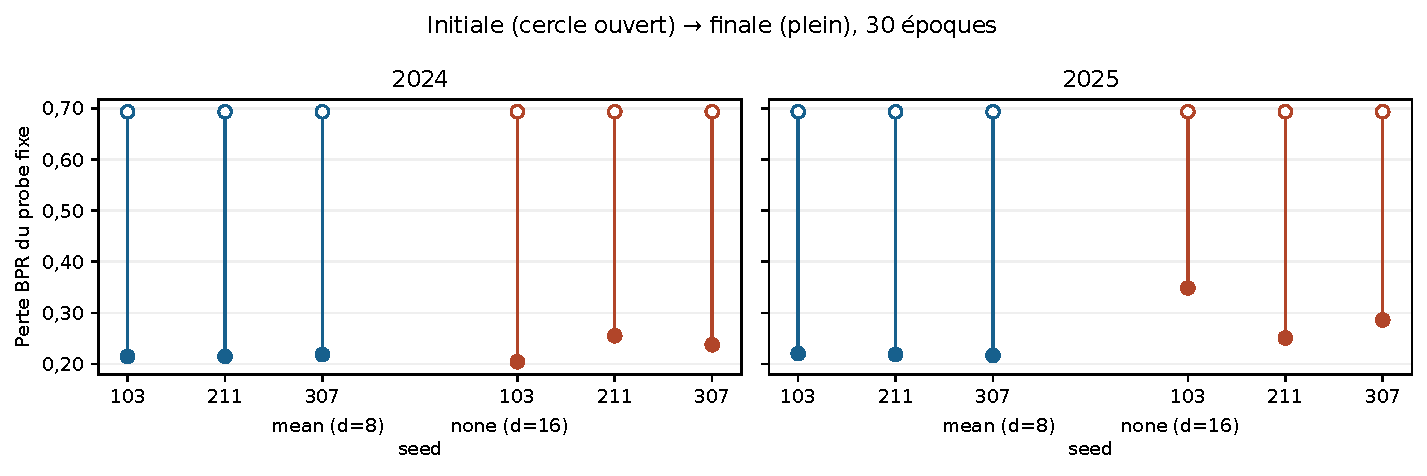
\includegraphics[width=\linewidth]{figures/q2_maude_learning_fr.pdf}
\caption{MAUDE Q2 : pertes avant/après sur le probe fixe d'apprentissage pour les 12 refits GraphSAGE sélectionnés (\emph{mean}/\emph{none}, tests 2024/2025, trois seeds chacun). Il s'agit de deux mesures du probe, avant puis après l'entraînement, pas de trajectoires de perte par époque.}
\label{fig:q2-maude-learning}
\end{figure}

\begin{figure}[!htbp]\centering
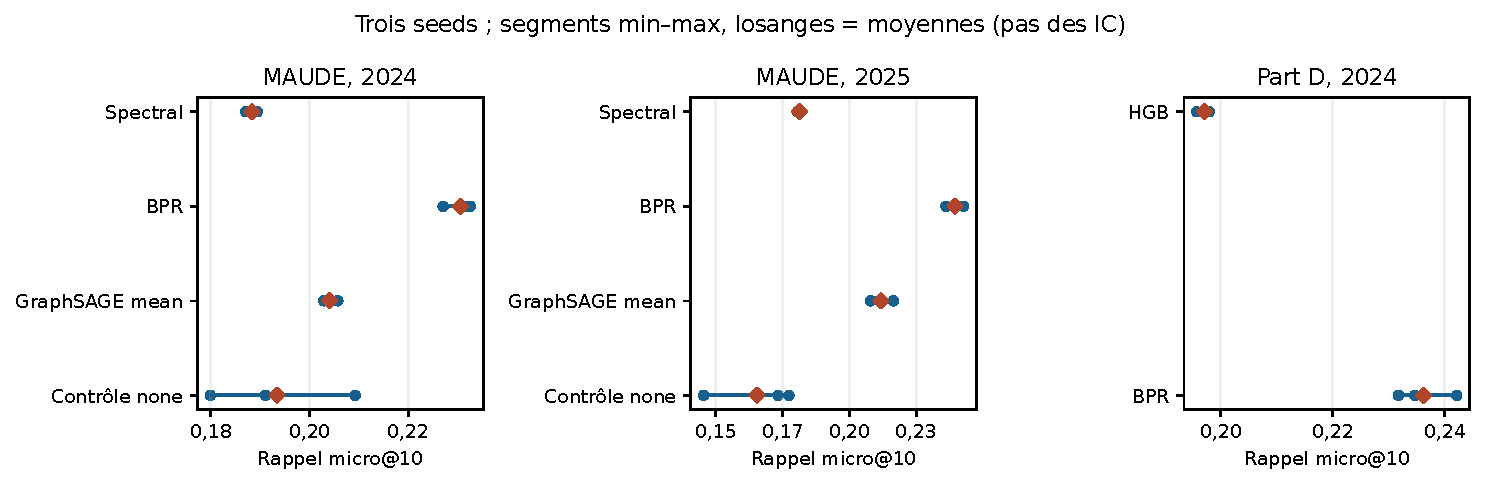
\includegraphics[width=\linewidth]{figures/q2_seed_sensitivity_fr.pdf}
\caption{Points des trois seeds et étendues min--max du rappel micro@10 pour MAUDE 2024--2025 et Part D 2024; aucune barre ne représente un intervalle de confiance ni un bootstrap.}
\label{fig:q2-seed-sensitivity}
\end{figure}

Aucun nouvel intervalle de confiance, test de significativité ou bootstrap n'est associé aux tableaux et figures Q2. Les trois seeds décrivent une sensibilité à l'entraînement, mais leurs étendues ne constituent pas des intervalles d'incertitude d'échantillonnage, de sélection ou d'entraînement. Les mesures de ressources ne sont pas comparables comme budgets égaux : les phases partagent la machine, et dimensions, répétitions et temps nécessaires varient.

\par\Needspace{12\baselineskip}
\section{Forecast Part D scellé et disponibilité future}
\label{supp:q2-prospective}

\textbf{Objet du forecast.} Le protocole Q2 définit une prévision d'une nouvelle relation observée dans la prochaine publication officielle annuelle Part D, pas une prédiction clinique de l'année de service 2025 ni d'une première prescription. L'origine scellée est une capture publique contemporaine des entrées effectivement employées; elle ne reconstitue pas leur disponibilité au cours des années de service 2019--2024 et ne sera pas recréée au moment de la publication de la cible\cite{hgbq2forecast}.

Le run \src{partd-prospective-001} a recapturé intégralement, sans authentification, les six CSV publics 2019--2024 : 22\,609\,355\,460 octets au total, avec SHA-256 enregistrés et concordant avec les fichiers locaux conservés. Le scellement de l'origine est intervenu le 3 octobre 2026 à 22:10:50.231060 UTC; le forecast final a été scellé à 22:28:54.610343 UTC. Le record d'origine porte le SHA-256 \src{ff6641fd17742aad670ed41748cd104e3bed058a65348459c390a716bda44fe3}; le forecast le SHA-256 \src{382e111529f4009c0790267d1518dab050f66d72badc2cb28c8acf2bc120ff9e}. Les corps du catalogue capturés avant les fits, après les recaptures et avant scellement ne listaient aucun nœud officiel de service 2025.

La cohorte déterministe contient 2\,000 NPIs présents dans l'historique avant la cible. Elle exclut l'union des 2\,518 NPIs des populations de développement et les 2\,288 du nouveau comparatif Part D, déjà inclus dans cette union. Le choix et la procédure de hachage sont scellés sans examiner les drugs, claims ou labels de la cible. Les configurations issues de la validation 2023 du comparatif sont reprises sans nouveau réglage ni choix de seed. Sept fits appris et deux heuristiques produisent chacun 2\,112\,688 scores de candidats; les trois seeds sont utilisés pour le HGB, car son entraînement comporte 359\,300 lignes, strictement au-dessus du seuil de 200\,000. Les 19 phases sur 19 sont achevées (2\,241{,}490 s de durée murale observée, RSS agrégée maximale de 834\,887\,680 octets). Ni label ni métrique de test 2025 ne figure dans ce forecast.
Après exclusions, le pool des NPIs apparus avant la cible compte 1\,490\,683 identifiants.
La sélection des 2\,000 identifiants suit l'ordre hexadécimal de \texttt{SHA256(salt + NUL + NPI)}, puis de NPI, avec le salt \texttt{q2-prospective-20261003}; le SHA-256 de la liste scellée est \src{2ec15e00cb4e90a390b6f668a0637cf250953ceb1ee7adb40334f7e626790319}.
Le vocabulaire de candidats reste celui déjà observé dans l'histoire 2019--2024; le forecast porte sur une relation nouvelle au sens des fichiers publiés, absente de l'historique du provider, et non sur une première prescription clinique ou un médicament inédit.

Des NPIs disjoints ne garantissent pas l'indépendance statistique des observations : médicaments, spécialités et dépendances de réseau peuvent être partagés. Le forecast applique une procédure fixée avec réajustement sur la seule histoire pré-cible de la nouvelle cohorte; il ne s'agit pas du transfert sans adaptation d'un checkpoint ancien.

Les empreintes des records scellés, dont celles des neuf fichiers de scores et des sept checkpoints appris, ont été ancrées dans le commit public GitHub \href{https://github.com/carabistouflette/HealthGraphBench/commit/2a59324003fe8b9c89a5f1e9ff6464f2a76f6ab2}{\nolinkurl{2a59324003fe8b9c89a5f1e9ff6464f2a76f6ab2}}. La visibilité publique du dépôt a été observée; le seul horodatage GitHub du commit n'est pas pris comme preuve de visibilité. Après cet ancrage, un nouveau catalogue public capturé le 3 octobre à 22:43:54.412446 UTC ne listait toujours pas le nœud annuel 2025. Cette capture atteste seulement l'état observé de ce catalogue à ce moment, non l'absence de données privées ou de toutes autres copies.
La réponse de catalogue postérieure à l'ancrage est archivée avec son corps exact : HTTP 200, 278\,033 octets, SHA-256 \src{1388b6cd63fd11d2977cb041d7ade58075b34ef3943253129b1df696325d85fa}; ce résultat atteste seulement la requête publique horodatée.

\textbf{Statut d'évaluation.} Le résultat demeure \texttt{sealed\_awaiting\_official\_target\_publication}. La source annuelle officielle 2025, ses labels et une métrique cible n'existent pas dans les preuves capturées; l'évaluation indépendante n'a pas passé. L'attestation humaine de non-consultation reste \texttt{unknown}. Le scellement et l'ancrage des scores ne remplacent ni la source cible ni les attestations humaines; aucune nouvelle origine n'est attribuée à l'année de service.

\subsection{Conditions d'une évaluation différée}

Une évaluation ultérieure ne pourra commencer qu'après observation du nœud officiel annuel 2025 dans le catalogue et de son média primaire. L'identifiant doit désigner le nœud annuel 2025, et non le terme de taxonomie partagé. Les métadonnées du média doivent établir une correspondance exacte de taille et de SHA-1 avec le CSV exposé par le média primaire; les octets doivent ensuite être recapturés publiquement et vérifiés contre le fichier cible local et son SHA-256. Une date HTTP, Drupal, modification, re-publication ou une mention d'année de service ne prouve pas la disponibilité historique d'octets identiques. Les labels ne sont évalués qu'avec les scores déjà scellés, sans réentraînement, réglage ou choix de seed; les conditions de non-consultation et attestations humaines requises doivent être réellement fournies. La date future de publication n'est pas connue et l'origine scellée n'est pas déplacée à cette date.

Les records scellés et les empreintes des scores sont inclus sous \src{data/q2/}; les neuf flux complets de scores restent dans l'archive prospective distincte. La provenance de capture figure dans \src{q2_partd_prospective_20261003.json}, \src{q2_partd_prospective_publication_20261003.json} et \src{q2_partd_prospective_publication_catalog_20261003.json}. Le contrôle post-publication conserve le corps exact du catalogue; il ne transforme pas une absence observée en preuve générale d'absence.

\par\Needspace{12\baselineskip}
\section{Migration de l'API Part D et réutilisation technique}
\label{supp:q2-reuse}

La migration remplace les anciens chemins actifs de lecture de rankings de model-gate par une API qui permet de charger une tâche, de lire son historique strictement antérieur et de faire réellement \texttt{fit\_predict}, produire des scores et recalculer les métriques via \texttt{PartDTask.evaluate}. \texttt{PartDTask.from\_model\_gate} et \texttt{load\_task(..., model\_gate\_dir=...)} ne sont plus des API actives. Les exemples de replay conservés dans le README sont historiques; ils ne décrivent pas cette nouvelle interface. L'API expose par \texttt{PartDHistoryView} les médicaments/providers du passé, les spécialités récentes, les candidats et le soutien, sans labels cibles; le scorer doit retourner un score fini pour chacun des candidats sans modifier la liste\cite{hgbq2methods}.

Le modèle nouveau \texttt{NeighborCosineTop50} est implémenté hors paquet. Il ajuste une incidence binaire provider--nom générique, calcule une similarité cosinus, retient au plus 50 voisins par provider en excluant soi-même et départage les égalités par NPI. Le score cumule les similarités des voisins qui ont observé le médicament candidat. Aucun paramètre, seed ou label de la cible n'est choisi; il s'agit d'un ajustement non supervisé, sans perte d'optimiseur à inventer. Les ajustements aux cutoffs 2023 et 2024 sauvegardent des checkpoints NPZ; après rechargement, l'identité des scores est vérifiée sur les listes de contrôle de 1\,004 et 1\,038 candidats respectivement, non sur un nouveau scoring intégral.

\begin{table}[!htbp]\centering\small
\caption{Témoignage de réutilisation raw--ajustement--scores--évaluation : le modèle cosine externe n'est pas réglé; la logistique SDK conserve l'algorithme historique à 18 époques et ne correspond pas au gagnant LBFGS de la grille Q2.}
\label{tab:q2-reuse}
% Derived from completed Q2 JSON; no new numerical experiment.
\begin{tabularx}{\linewidth}{@{}Xrr@{}}
\toprule
Méthode & Val. 2023 & Test 2024 \\
\midrule
Cosine top50 hors paquet & $0{,}260960$ & $0{,}258583$ \\
Logistique SDK (18 époques) & $0{,}178460$ & $0{,}168188$ \\
\bottomrule
\end{tabularx}

\end{table}

Le parcours a été effectué dans un wheel construit depuis un clone propre au commit \src{f8ea41c4d8f090560fbdbc698db2300821b9cfef}; le wheel de développement de version 0.2.0 a le SHA-256 \src{b5c776556ef64686804c4dec6e354127c59c3db441710519da793ffee6117428}. Le driver isolé utilise \texttt{python -I} depuis sa phase, les 40 fichiers de package vérifiés dans \texttt{site-packages} et aucun environnement editable, \texttt{PYTHONPATH} ou patch de whitelist. Les six CSV ont été vérifiés, une préparation fraîche a été produite, cosine et véritable logistique publique ont été ajustés, tous les candidats ont été scorés et l'évaluation a été recalculée. En test 2024, 981 providers sur 2\,000 n'ont aucun positif; ils restent inclus dans la charge. La logistique SDK à 18 époques n'est pas le comparateur logistique LBFGS choisi sur validation dans la grille Part D Q2; ces résultats servent à constater la réutilisation technique, pas à ajouter une comparaison réglée.

Les commandes de reconstruction s'exécutent dans un clone du dépôt original, pas depuis les fichiers vendored de lecture. Le commit de provenance du snapshot RC3 est \src{6b4ae00ebc4b701d757260616ccb0df16f51467b}; chaque run publié garde aussi son propre commit de code exécuté (S12). Il faut fournir les raw utilisateur correspondant aux manifestes, vérifier leurs empreintes, copier le protocole exact livré sous \src{data/q2/} et choisir un répertoire de sortie neuf. Le dépôt compact ne contient pas les flux raw complets. Exemple d'un clone et de variables à adapter aux fichiers effectivement acquis :

\begin{Verbatim}[fontsize=\footnotesize]
git clone https://github.com/carabistouflette/HealthGraphBench.git q2-original
git -C q2-original checkout 6b4ae00ebc4b701d757260616ccb0df16f51467b
cd q2-original
Q2_PROTOCOL=/path/to/HealthGraphBench_RC3/data/q2/q2_scientific_protocol_20261003.json
Q2_PROTOCOL_SHA256=22b3b308e1ddd55f9ebfc388edc1a08ba3dc8a4a83205b230406643155536db7
python scripts/run_q2_maude.py --source-root "$MAUDE_RAW" \
  --protocol "$Q2_PROTOCOL" --protocol-sha256 "$Q2_PROTOCOL_SHA256" \
  --output-dir NEW/maude
python scripts/run_q2_cms.py --source-root "$CMS_RAW" \
  --protocol "$Q2_PROTOCOL" --protocol-sha256 "$Q2_PROTOCOL_SHA256" \
  --output-dir NEW/cms
python scripts/run_q2_partd.py --source-root "$PARTD_RAW" \
  --protocol "$Q2_PROTOCOL" --protocol-sha256 "$Q2_PROTOCOL_SHA256" \
  --output-dir NEW/partd
\end{Verbatim}

La reprise MAUDE est un chemin distinct qui exige la validation complète archivée et la même racine raw, pas une nouvelle grille :

\begin{Verbatim}[fontsize=\footnotesize]
python scripts/run_q2_maude.py --complete-validation ROOT001 \
  --source-root "$MAUDE_RAW" --protocol "$Q2_PROTOCOL" \
  --protocol-sha256 "$Q2_PROTOCOL_SHA256" --output-dir NEW/maude-completion
\end{Verbatim}

Le calcul original du forecast utilisait le comparatif Part D achevé et les CSV raw. La commande ci-dessous documente ce chemin : une nouvelle exécution aurait une nouvelle origine et ne remplacerait pas les scores scellés. L'évaluation différée doit utiliser les sorties originales conservées, sans refit :

\begin{Verbatim}[fontsize=\footnotesize]
python scripts/run_q2_prospective_partd.py forecast \
  --source-root "$PARTD_RAW" --comparison-dir "$PARTD_COMPARISON" \
  --protocol "$Q2_PROTOCOL" --protocol-sha256 "$Q2_PROTOCOL_SHA256" \
  --output-dir NEW/partd-prospective
\end{Verbatim}
Pour le témoin raw--wheel de réutilisation, utiliser également un interpréteur du wheel propre vérifié et une destination neuve :

\begin{Verbatim}[fontsize=\footnotesize]
python scripts/run_q2_reuse.py --source-root "$PARTD_RAW" \
  --protocol "$Q2_PROTOCOL" --protocol-sha256 "$Q2_PROTOCOL_SHA256" \
  --output-dir NEW/reuse --reuse-python "$REUSE_PYTHON"
\end{Verbatim}

Les archives d'expériences restent distinctes du ZIP compact du manuscrit : MAUDE 141\,798\,509 octets (SHA-256 \src{dbce2d88f335b0b718d2decc750dae2638f6de877e8542fb93857a6691a0d637}), CMS 4\,569\,115 octets (\src{a11d34e9946c6c03b4b092a423d421094b808db8067ab30777eb2f6b1751cb80}), Part D 630\,693\,314 octets (\src{abaf9d40356dc6a8dc02cdddc5fa70328f9e18d082f7f2fabc0989328de3fca4}), réutilisation 13\,086\,403 octets (\src{b0b2cddc54be88120dc6933f544cfa5d4be3811b77d1b65bb15a5e403c66315a}) et forecast prospective 115\,004\,400 octets (\src{ced58e93d6168e6767bbbf34d6eb9a5785b4e8279ea59f012749c1aba474d35c}). Les archives MAUDE/CMS/Part D/réutilisation/forecast n'incluent pas les raw sources; le paquet compact RC3 ne prétend donc pas contenir les 193 checkpoints des comparaisons, les neuf fichiers complets de scores prospectifs ni les flux Q2 complets. Ces artefacts demeurent dans les archives externes indexées par leurs ledgers et empreintes; les vrais raw doivent être fournis par l'utilisateur depuis les sources prescrites et vérifiés avant exécution.

Les rapports de vérification sont référencés dans \src{data/q2/q2_runtime_verification_20261003.json} et \src{data/q2/q2_prospective_software_preflight_20261003.json}. Le premier consigne 80 tests logiciels sans échec; les checks de chargement du wheel et le prévol du contrôleur restent des preuves de logiciel, pas une validation scientifique externe. Le prévol prospectif utilise 4\,000 identifiants synthétiques et des médicaments fictifs; ses rappels@10 = 0{,}5 et @20 = 1,0 démontrent seulement le chemin de calcul sur fixture. Ils ne sont ni une source médicale ni un résultat de modèle de santé. La réutilisation effective a été exécutée par un assistant/agent : aucune étude par participant humain extérieur n'a été réalisée et cette gate demeure en attente. Les noms/auteurs, affiliations, déclarations et approbations humaines restent à établir séparément.
